\section{RankState Struct Reference}
\label{structRankState}\index{RankState@{RankState}}
{\tt \#include $<$cmd\_\-issuer.h$>$}

Collaboration diagram for RankState:\nopagebreak
\begin{figure}[H]
\begin{center}
\leavevmode
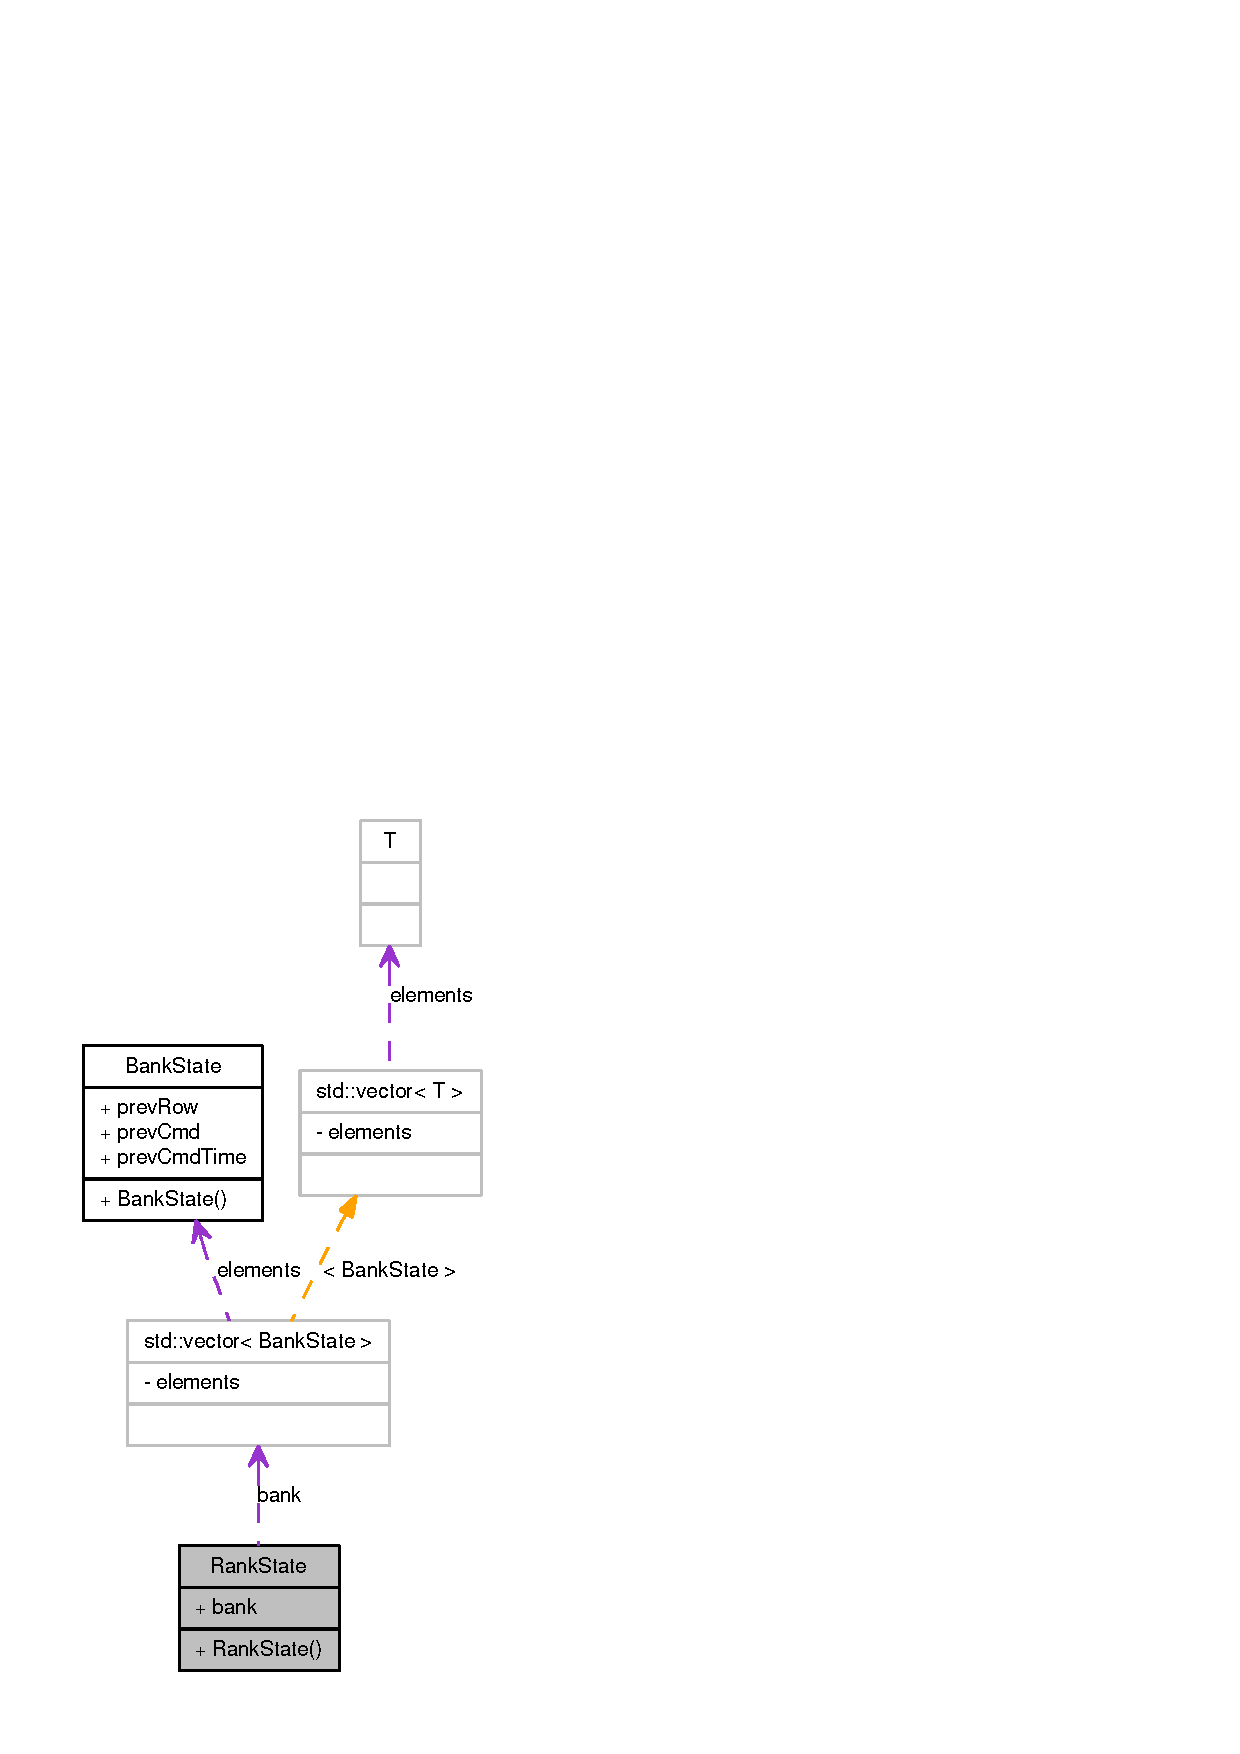
\includegraphics[height=400pt]{structRankState__coll__graph}
\end{center}
\end{figure}
\subsection*{Public Member Functions}
\begin{CompactItemize}
\item 
{\bf RankState} ()
\end{CompactItemize}
\subsection*{Public Attributes}
\begin{CompactItemize}
\item 
vector$<$ {\bf BankState} $>$ {\bf bank}
\end{CompactItemize}


\subsection{Detailed Description}


Definition at line 90 of file cmd\_\-issuer.h.

\subsection{Constructor \& Destructor Documentation}
\index{RankState@{RankState}!RankState@{RankState}}
\index{RankState@{RankState}!RankState@{RankState}}
\subsubsection[{RankState}]{\setlength{\rightskip}{0pt plus 5cm}RankState::RankState ()\hspace{0.3cm}{\tt  [inline]}}\label{structRankState_56184cca248259f03cd7dc2de0f495fc}




Definition at line 93 of file cmd\_\-issuer.h.

References bank, and NO\_\-OF\_\-BANKS.

\subsection{Member Data Documentation}
\index{RankState@{RankState}!bank@{bank}}
\index{bank@{bank}!RankState@{RankState}}
\subsubsection[{bank}]{\setlength{\rightskip}{0pt plus 5cm}vector$<${\bf BankState}$>$ {\bf RankState::bank}}\label{structRankState_3bccebe16e7c088968aee892cdfea434}




Definition at line 92 of file cmd\_\-issuer.h.

Referenced by RankState().

The documentation for this struct was generated from the following file:\begin{CompactItemize}
\item 
{\bf cmd\_\-issuer.h}\end{CompactItemize}
